\documentclass[10pt,a4paper]{article}
\usepackage[latin1]{inputenc}
\usepackage{amsmath}
\usepackage{amsfonts}
\usepackage{amssymb}
\usepackage{graphicx}
\author{Lucas Swartsenburg}
\title{Takehome2}

\begin{document}
\maketitle
\section*{1a}
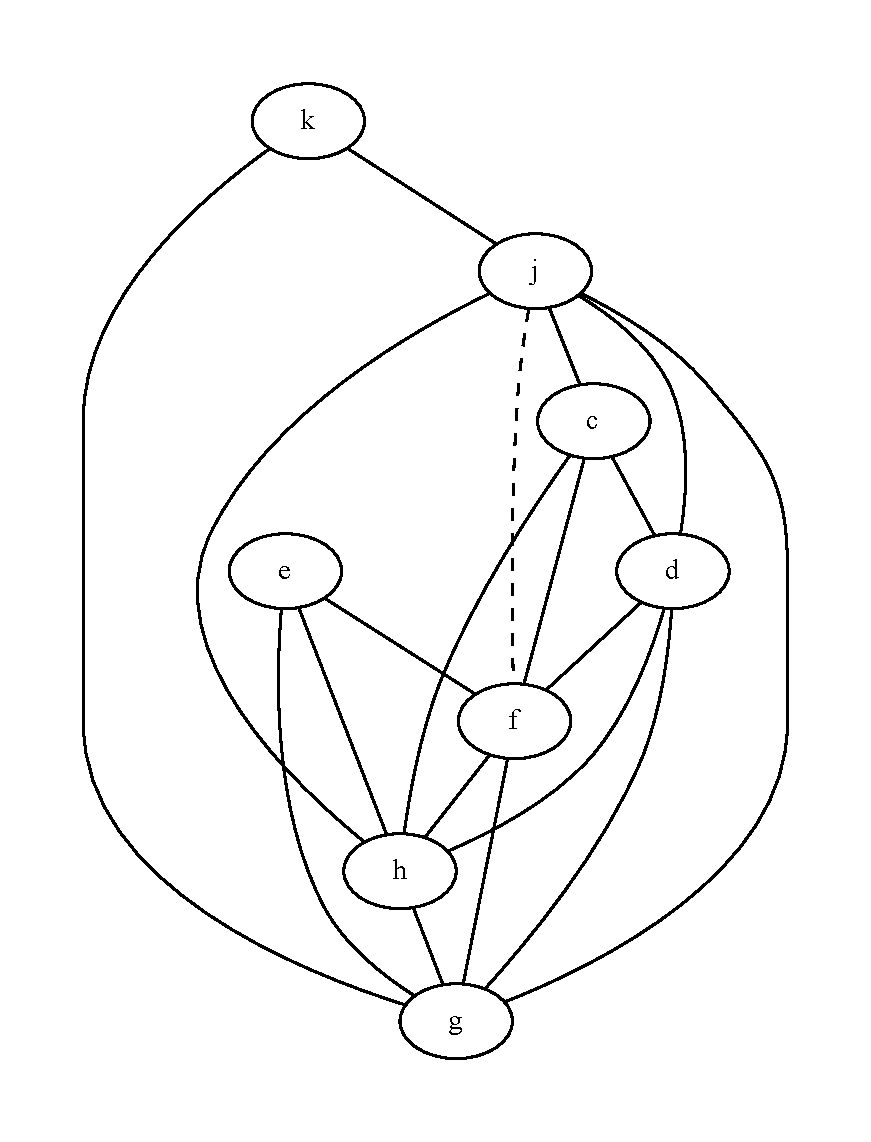
\includegraphics[scale=0.8]{interference.pdf} 
\section*{1b}
\begin{verbatim}
    We kleuren voor 4 registers dus K = 4
    Stap 1
        stack (top links): leeg

        'k' heeft maar 2 neighbours.
        simplify met 'k' (haal k en zijn edges weg en zet op stack)

    Stap 2
        stack: k

        'e' heeft maar 3 neighbours.
        verwijder 'e' van graph.

    Stap 3
        stack: e, k

        Er zijn geen nodes met minder dan K neighbours
        we moeten spillen.
        Spill 'h' (verwijder 'h' en edges naar, en zet op de stack gemarkeerd
        als gespilde node).

    Stap 4
        stack: h (S), e, k

        'c' heeft maar 3 neighbours.
        simplify met 'c'.

    Stap 5
        stack: c, h (S), e, k

        'g' heeft maar 3 neighbours.
        simplify met 'g'.

    Stap 6
        stack: g, c, h (S), e, k

        'd' heeft maar 2 neighbours.
        simplify met 'd'.

    Stap 7
        stack: d, g, c, h (S), e, k

        Alleen 'j' en 'f' zijn nu nog over
        en zij hebben een move gemeen zonder tegelijk alive te zijn,
        we kunnen 'j' en 'f' dus tot 1 node omzetten. Verder
        kunnen we de move verwijderen.

    Stap 8
        stack: d, g, c, h (S), e, k

        'j&f' heeft 0 neighbours dus we kunnen simplifyen
        Nu is de graaf leeg.

    Stap 9
        stack: j&f, d, g, c, h (S), e, k

        We kunnen beginnen met selecten en colouren door van de
        stack te poppen. We zullen steeds proberen de laagst
        mogelijk vrije kleur te kiezen.

        We gebruiken:
            R0 - rood
            R1 - groen
            R2 - blauw
            R3 - geel
            spilled - geen kleur

        Pop 'j&f' en geef het R0.

    Stap 10
        stack: d, g, c, h (S), e, k

        Pop 'd' en geef het R1.

    Stap 11
        stack: g, c, h (S), e, k

        Pop 'g' en geef het R2.

    Stap 12
        stack: c, h (S), e, k

        Pop 'c' en geef het R2.

    Stap 13
        stack: h (S), e, k

        Pop 'h', h was spilled, maar we kunnen hem zowaar
        kleuren, geef het R3.

    Stap 14
        stack: e, k

        Pop 'e' en geef het R1.

    Stap 15
        stack: k

        Pop 'k' en geef het R1.

    De graaf is nu volledig gekleurd.
\end{verbatim}

\end{document}